\documentclass[a4paper,11pt,twoside]{scrreprt}

\usepackage{txfonts}
\usepackage{graphicx}
\usepackage[utf8]{inputenc}
\usepackage[ngerman]{babel}
\usepackage[T1]{fontenc}
\usepackage{user} % eigene Befehle

\ifpdf
  \usepackage[ps2pdf]{thumbpdf}
  \usepackage[pdftex]{hyperref}
\else
  \usepackage[active]{srcltx}
\fi

\newcommand{\dctitle}{Literaturverwaltung}
\newcommand{\dcsubject}{Projektdokumentation}
\newcommand{\dcsubtitle}{Teilbeleg 1}
\newcommand{\dcauthor}{Simon Wunderlich}
\newcommand{\dcdate}{\today}

\ifpdf
\hypersetup{%
   pdfauthor={\dcsubject - \dcauthor}
   pdftitle={\dctitle}
   bookmarksnumbered=true,
   pdfstartview={FitH},
   colorlinks=true,
   linkcolor=black,
   plainpages = false
}
\fi
 % Metainformationen wie Titel, Autoren,...

\begin{document}
% Momentan (schlecht) handgestrickt - wenn jemand es mit \maketitle und den
% Autoren wie in Vorlage hinbekommt, bitte ändern

\begin{titlepage}
	\begin{center}
		\vfill
		{% Kopf des Titels
			\large Softwarepraktikum 2006\\[1.5ex]
		}
		\vfill \vfill

		%Titel
		\textbf{\Huge\dctitle}
		\vspace{1.5cm}
		
		% Subjekt
		\textbf{\Large\dcsubject}

		% Untertitel
		\textsc{\Large \dcsubtitle}
		\vfill \vfill
	\end{center}
	
	
	{%Autoren
		\begin{tabbing}
			\hspace{4.5cm}\=\textbf{Teamleiter:}\hspace{0.5cm}\=Simon~Wunderlich\\[2.0ex]
				\>\textbf{Mitglieder des Projektteams:}\\[1.5ex]
				\>            \>Andreas~Tröger \\[1.5ex]
				\>            \>Benedikt~Keil \\[1.5ex]
				\>            \>Frank~Wilhelm \\[1.5ex]
				\>            \>Florian~Scharl \\[1.5ex]
				\>            \>Sven~Eckelmann \\[4.0ex]
				\> \textbf{Praktikumsbetreuer:} Michael Rentzsch
		\end{tabbing}
	}
	\vfill
	
	{%Betreuer
		Chemnitz, den \dcdate
	}
\end{titlepage}
 % Titel des Dokuments mit Informationen aus meta

% nur zum arbeiten
\tableofcontents

%Kapitel
\chapter{Spezifikation der funktionellen Anforderungen}
\section{Produktbeschreibung}
TODO: Blablabla, alles wichtig und ganz toll

\section{Funktionelle Anforderungen}
\subsection{Umgebungsmodell}

\subsubsection{Ereignistabelle}
%wenn die Tabellen zu lang werden -> longtable
TODO:
\begin{tabular}[ht]{|l|l|l|l|}
\hline
Nr & Ereignis & Datenfluß im System & Antwort des Systems \\
\hline\hline
1. & A ändert oder Ergänzt Bucherliste & Bücherdaten & Bestätigung\_Bücheränderung \\
2. & B macht auch was & Zahlungen & Ignorieren\_Änderungen \\
2. & B macht auch was & Zahlungen & Ignorieren\_Änderungen \\
2. & B macht auch was & Zahlungen & Ignorieren\_Änderungen \\
\hline
\end{tabular}

\subsubsection{Kontextdiagramm}
TODO
%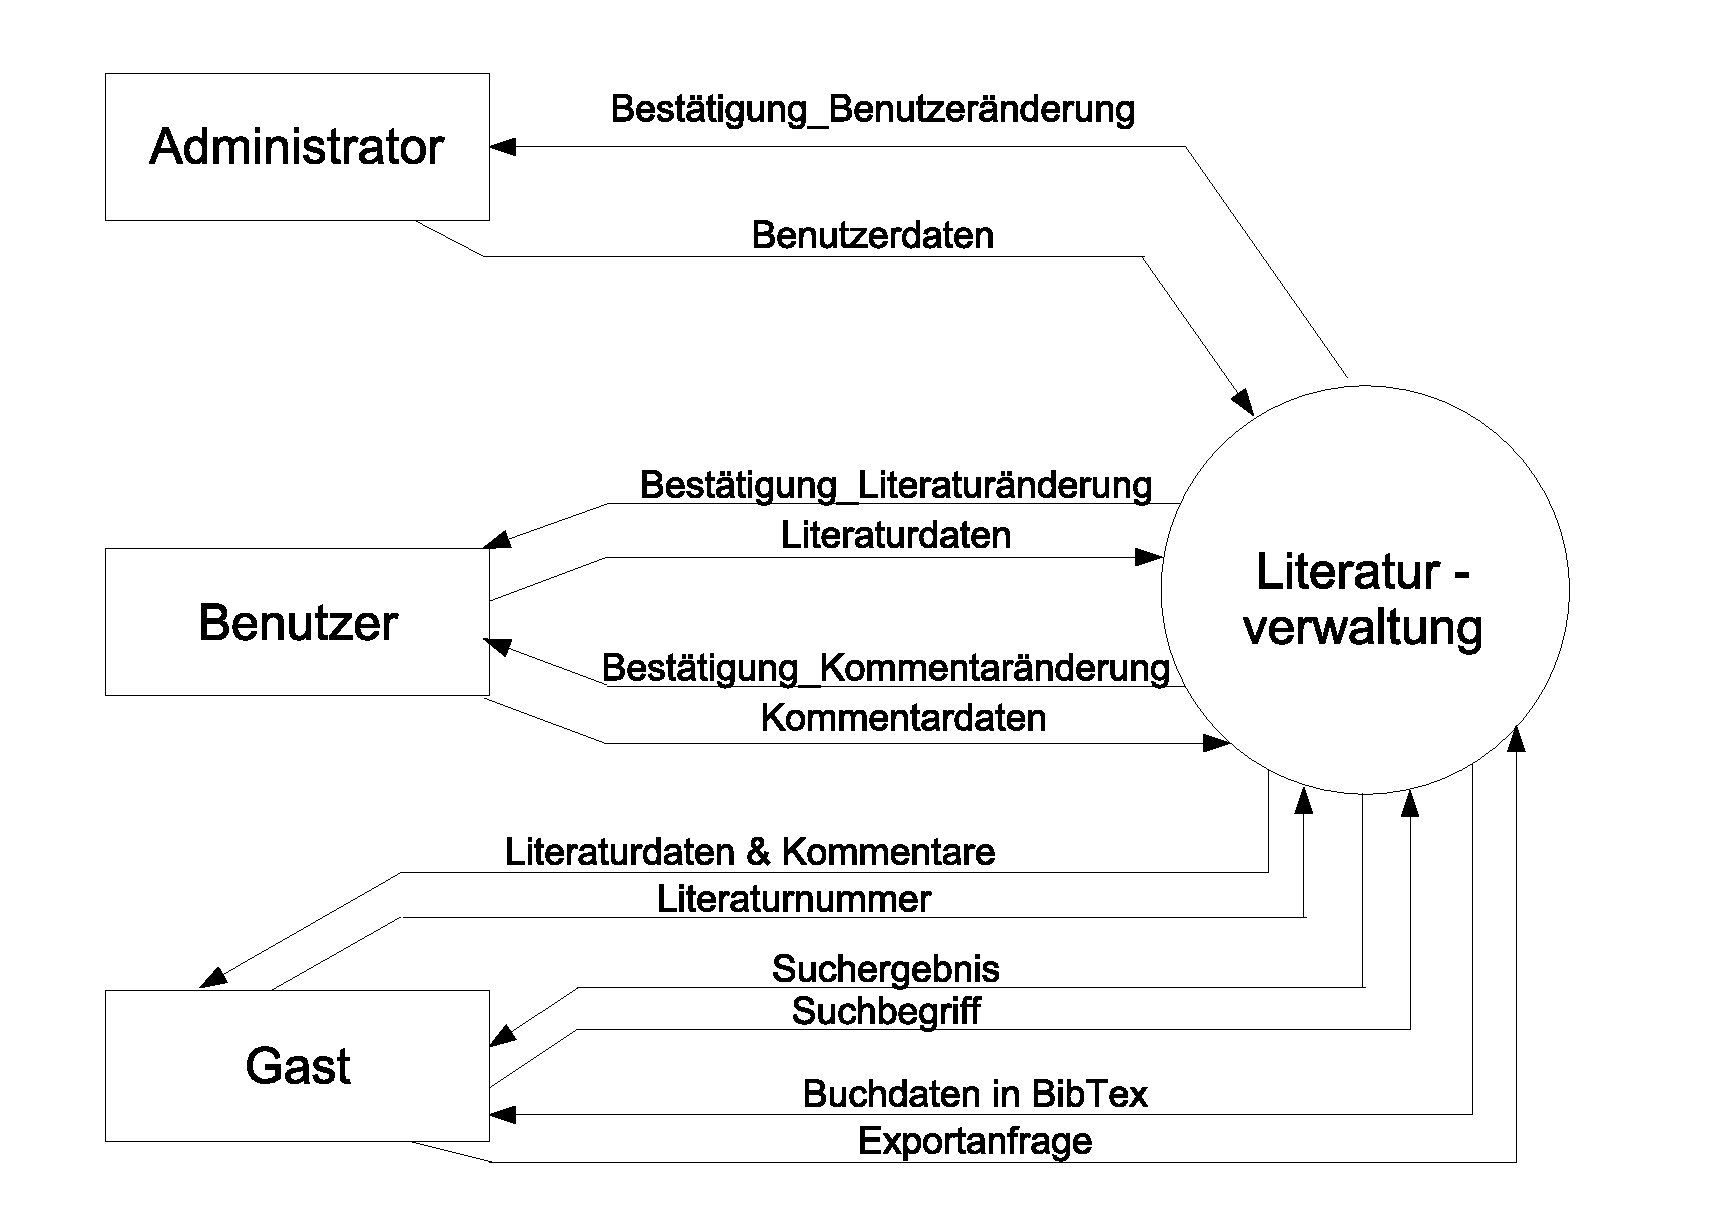
\includegraphics[scale=0.5]{kontextdiagramm}
% oder \centerline{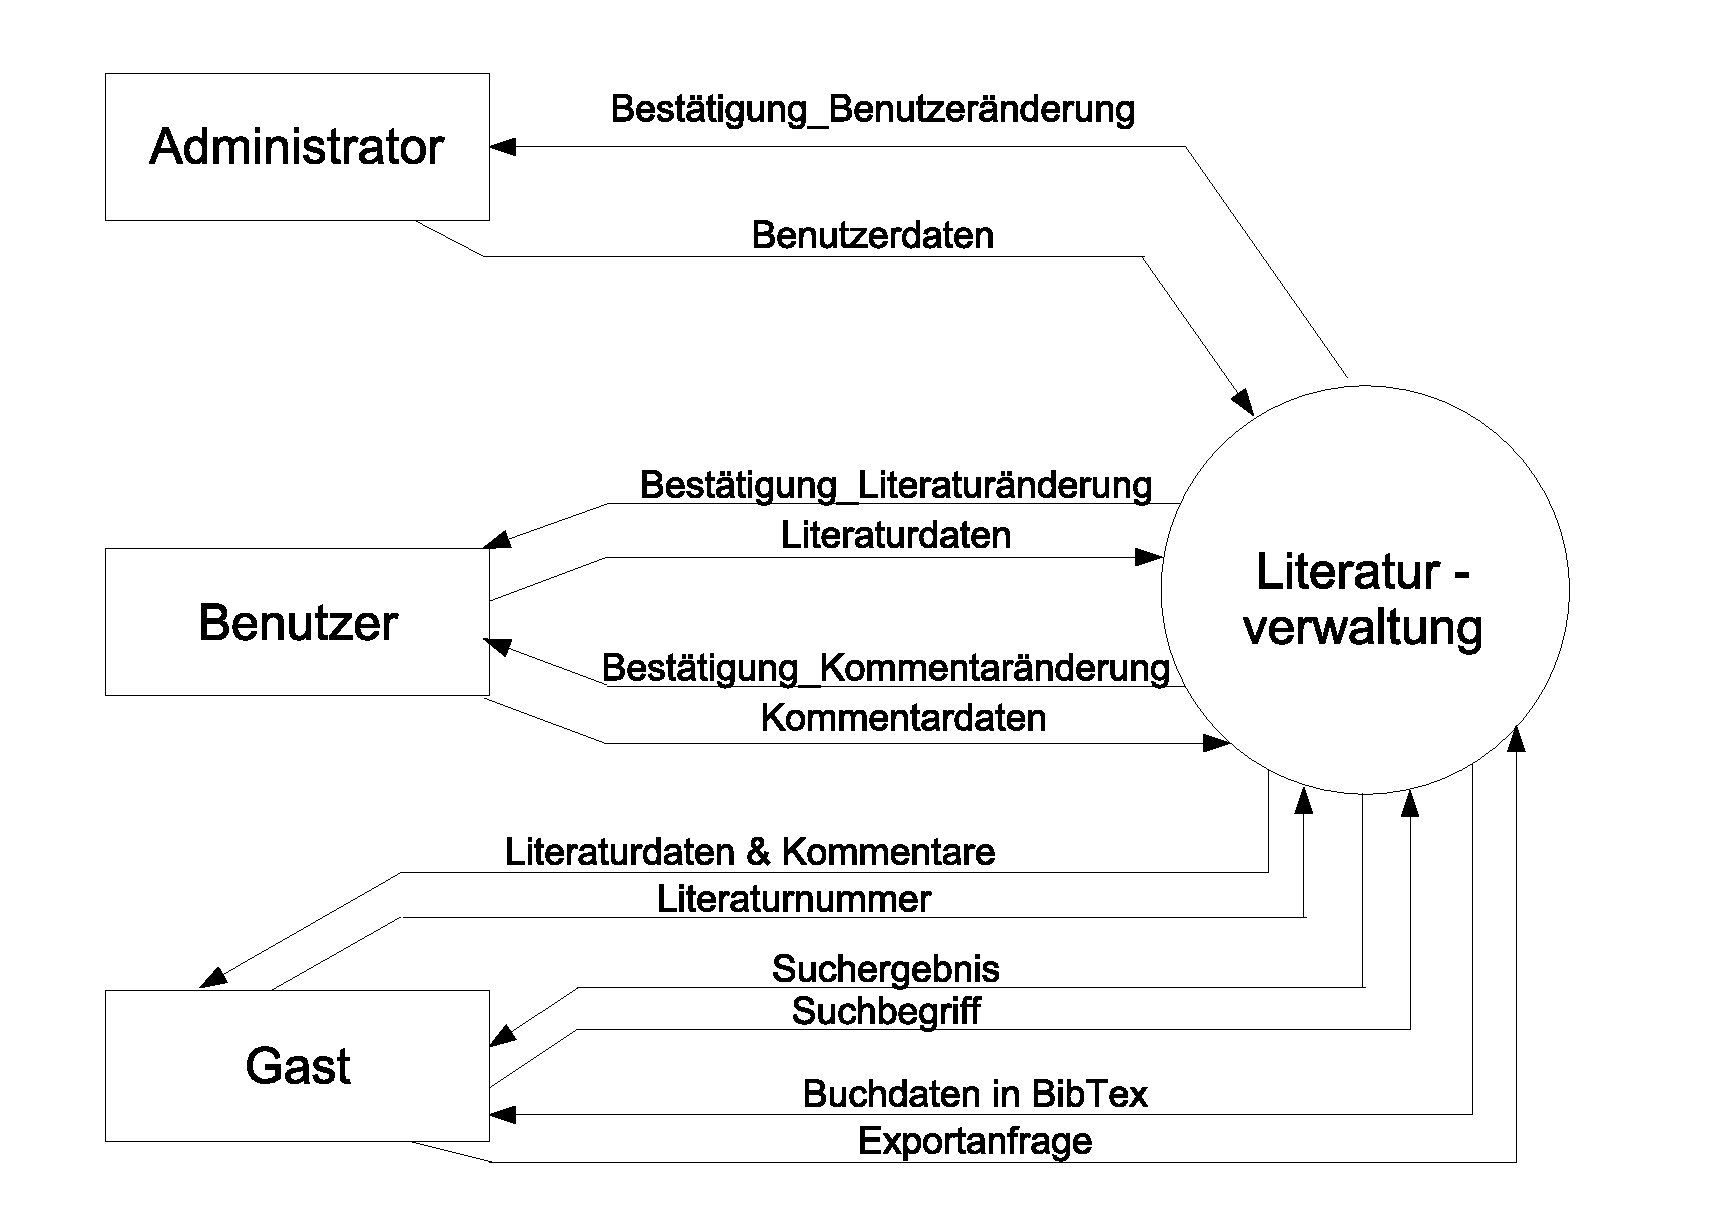
\includegraphics[scale=0.5]{kontextdiagramm}}

\subsection{Verhaltensmodell}
\subsubsection{Grobes Verhaltensmodell (vergröbertes primäres Verhaltensmodell)}
TODO
%\includegraphics[scale=0.5]{verhaltensmodell_grob}

\subsubsection{Primäres Verhaltensmodell}
\paragraph{Teilmodell blabla}
TODO
%\includegraphics[scale=0.5]{erhaltensmodell_blabla}

\paragraph{Teilmodell bloblo}
TODO
%\includegraphics[scale=0.5]{verhaltensmodell_bloblo}

\subsubsection{Verfeinerungen der Prozesse des primären Verhaltensmodells}
\paragraph{Verfeinerung zum Prozess: ieeekks}
TODO
%\includegraphics[scale=0.5]{prozess_ieeekks}

\paragraph{Verfeinerung zum Prozess: arrgghhh}
TODO
%\includegraphics[scale=0.5]{prozess_arrgghhh}

\subsubsection{Datenkatalog}
TODO:
\begin{tabular}[ht]{|l|l|}
\hline
Element & Strukturbeschreibung \\
\hline\hline
% Mitglieder
\emph{Mitglieder} & \{Mitglied\} \\
Mitglied  & M\_Name + Anschrift + <Beitritts>Datum + @Parzellen\_Nr + (Funktion) \\
\hline\hline
\emph{Leistungen} & {Leistung} \\
.... & ... \\
\hline
\end{tabular}

\subsubsection{Beziehungen zwischen Speichern (ERD)}
%wenn die Tabellen zu lang werden -> longtable
TODO:
%\includegraphics[scale=0.5]{erd}

\subsubsection{Prozessspezifikation}
TODO: (siehe Beispielbeleg S. 9)

\paragraph{Prozess abc}

\paragraph{Prozess cde}

\subsection{Definition der Nutzerschnittstelle}
TODO (Generell, Fargestaltung)

\subsubsection{Ein- und Ausgabegeräte}
TODO Siehe Beispielbeleg S. 11

\paragraph{Legende zur Layoutdarstellung}
TODO Siehe Beispielbeleg S. 11

\paragraph{Grundfenster}
TODO

\paragraph{Menüs}
TODO

\paragraph{Fenster irgendwas}
TODO
\chapter{Spezifikation der operationellen Anforderungen}
\section{Operationelle Anforderungen an die Daten und Datenbasen}
Für die Abschätzung des Speicherplatzbedarfes für Daten und Speicher wird von den Annahmen ausgegangen,
dass für die Speicherung von in der Regel (bis auf wenige Ausnahmen, für die das gesondert vermerkt ist)\\
         gZahl - 2Byte, rZahl - 4 Byte\\
         Zeichenkette - 1Byte pro Zeichen (der maximalen Länge) erforderlich sind.

TODO:
\begin{tabular}[ht]{|l|l|l|}
\hline
Element & Struktur & Bytes \\
\hline\hline
% Mitglieder
Mitglied  & M\_Name + (Funktion) & $50+14=64$ \\
M\_Name  &  <Vor>Name + <Familien>Name & $25+25=50$ \\
M\_Name  &  ["Vorsitzender" | "Stellvertreter" | "Kassenwart"] & $14$ \\
\hline\hline
Leistung & abc+cde & $19+23=42$ \\
.... & ... & ... \\
\hline
\end{tabular}

\subsection{Speicher (Angaben zum Speicherbedarf in Byte)}
TODO:
\begin{tabular}[ht]{|l|l|l|l|l|}
\hline
Speicher & Struktur & Minimum & Mittel & Maximum \\
\hline\hline
Mitglieder & {Mitglied} & $0*64$ & $50*64=3200$ & $100*64=6400$ \\
Leistungen & {Leistung} & $0*42$ & $50*42=2100$ & $100*42=4200$ \\
\hline
\end{tabular}

\subsection{Weitere Datenflüsse}
TODO:
\begin{tabular}[ht]{|l|l|l|l|l|}
\hline
Datenfluss & Struktur & Minimum & Mittel & Maximum \\
\hline\hline
Revisionsunterlagen & {Mitglied} & $0*64$ & $50*64=3200$ & $100*64=6400$ \\
\hline
\end{tabular}

\subsection{Abschätzungen}
TODO:
\begin{itemize}
 \item \textbf{Gesamtsystem}: blablabla
 \item \textbf{Mitglieder}: blub
 \item \textbf{Leistungen}: jaja
 \item \textbf{Revisionsunterlagen}: nicht die auch noch
\end{itemize}

\subsection{Genauigkeit}
TODO siehe Beispielbeleg S. 23

\section{Operationelle Anforderungen an die Datenströme}
TODO siehe Beispielbeleg S. 23

\section{Operationelle Anforderungen an die Prozesse}
TODO siehe Beispielbeleg S. 23
\chapter{Spezifikation wichtiger Qualitätsanforderungen}
\section{Benutzerbarkeit}
Im wesentlichen existieren drei Arten von Benutzern:

\begin{enumerate}
 \item \textbf{Administrator:}\\
Er ist im wesentlichen f\"ur die Mitgliedsverwaltung zust\"andig, also das Anlegen, \"Andern und L\"oschen von Mitgliedseintr\"agen. \\
Des Weiteren k\"ummert er sich mit Hilfe der quelloffenen Basisprogramme um Datensicherungen. Eine gewisse Grundkenntnis im Umgang mit
besagten Programmen ist also vorrausgesetzt.

 \item \textbf{Mitglied:}\\
Nachdem man in der Literaturverwaltung registriert ist, wird man zum Mitglied und erh"alt neue Nutzerprivilegien. \\
So kann man neue Literatur hinzuf\"ugen, ab\"andern und l\"oschen oder Kommentare \"uber Literatureintr\"age verfassen.

 \item \textbf{Nutzer:}\\
Wenn man sich nicht registriert, ist man in der Gruppe der Nutzer. Diese Gruppe hat keine M\"oglichkeit auf den Datenbestand der Literaturverwaltung einzuwirken.\\
Die Rechte sind auf die Recherche beschr\"ankt, der Nutzer kann also B\"ucher suchen, ausw\"ahlen und sich die Beschreibungen und Kommentare ansehen.
\end{enumerate}

\section{Zuverlässigkeit}
Eine einfache Bedienoberfl\"ache und klar formulierte Fehlermeldungen erm\"oglichen dem Nutzer bei Fehleingaben schnell auf die entsprechende Situation zu reagieren.\\
Daten, die gespeichert werden sollen, werden erst nach Best\"atigung in den Bestand \"ubernommen, sollte es vor der Best\"atigung zu einem Absturz kommen, muss das Mitglied die Daten erneut eingeben. \\
Sollte es zur unbeabsichtigten L\"oschung oder Besch\"adigung von Daten kommen, hat der Administrator au\ss erhalb des zu entwicklenden Systems M\"oglichkeiten mit Hilfe des verwendeten Datenbanksystems diese zu retten.

\section{Integrität}
Auch wenn aktiv auf den Datenbestand eingewirkt werden kann, so ist dies jedoch ausschlie\ss lich registrierten Mitgliedern m\"oglich solche \"Anderungen vorzunehmen.
Diese \"Anderungen k\"onnen auch vom Administrator bereinigt werden.\\
Sollte es wiederholt zu sch\"adigenden Eingriffen seitens eines Mitglieds kommen, so ist es dem Adminstrator möglich das betreffende Mitgliedskonto samt aller Mitgliedsdaten zu l\"oschen.

\section{Flexibilität}
Bereits im Datenbankentwurf wurde auf sp\"atere Modifikationen des Projekts seitens des Kunden R\"ucksicht genommen. Es wurden Schnittstellen zum Datenbestand implementiert die sp\"atere \"Anderungen wesentlich erleichtern. \\

\section{Portabilität}
Aufgrund der frei verfügbaren und verbreiteten Software, die zum Betrieb der Software benötigt werden, kann die Software auf einer großen Reihe von Hard- und Softwarekombinationen genutzt werden. Eine Benutzung anderer Basissoftware ist nicht direkt möglich.

\chapter{Basismaschine und Entwicklungsumgebung}
\section{Basismaschine}
\subsection{Hardwarekonfiguration}
TODO siehe Beispielbeleg S. 25\\
Als notwendige Minimalausstattung des für den Betrieb des Systems erforderlichen PCs werden angesehen:
\begin{itemize}
 \item Basis-PC
 \item Nadeldrucker
\end{itemize}


\subsection{Betriebssystem}
TODO siehe Beispielbeleg S. 25


\subsection{Sonstige Basissoftware}
TODO siehe Beispielbeleg S. 25


\section{Entwicklungsumgebung}
TODO siehe Beispielbeleg S. 26
\chapter{Planung}
\section{Gantt-Diagramm}
\includegraphics[scale = 0.93, bb = 1.5cm 14.8cm 19.4cm 28cm]{ganttchart}

\end{document}
